\documentclass[11pt,twocolumn,letterpaper]{article}

\usepackage{cvpr}
\usepackage{float}
\usepackage{times}
\usepackage{epsfig}
\usepackage{graphicx}
\usepackage{amsmath}
\usepackage{amssymb}
\usepackage{subcaption}

% Include other packages here, before hyperref.

% If you comment hyperref and then uncomment it, you should delete
% egpaper.aux before re-running latex.  (Or just hit 'q' on the first latex
% run, let it finish, and you should be clear).
\usepackage[breaklinks=true,bookmarks=false]{hyperref}

\cvprfinalcopy

\def\cvprPaperID{****} % *** Enter the CVPR Paper ID here
\def\httilde{\mbox{\tt\raisebox{-.5ex}{\symbol{126}}}}

% Pages are numbered in submission mode, and unnumbered in camera-ready
%\ifcvprfinal\pagestyle{empty}\fi
\setcounter{page}{1}
\begin{document}

%%%%%%%%% TITLE
\title{
    CS 388 Final Project Proposal:
    Seq2Seq Architecture Extension\\}

\author{Keivaun Waugh\\
ksw734\\
{\tt\small keivaun@protonmail.com}
% For a paper whose authors are all at the same institution,
% omit the following lines up until the closing ``}''.
% Additional authors and addresses can be added with ``\and'',
% just like the second author.
% To save space, use either the email address or home page, not both
}

\maketitle
%\thispagestyle{empty}

%%%%%%%%% ABSTRACT
\begin{abstract}
    Sequence to sequence models \cite{Seq2Seq} have shown much promise for performing translations, both literal translations between languages, and translations between structures. Coupled with attention mechanisms such as in \cite{LuongAttention} that help the decoder learn which input words to ``focus'' on, they can achieve state-of-the-art performance. For my final project, I propose an extension to the Seq2Seq architecture that may help the network learn more easily.
\end{abstract}

%%%%%%%%% BODY TEXT
\section{Motivation}
The motivation behind this project idea is to first transform the sentence to a parse of the sentence before attempting to do any kind of translation. By using a parse of the sentence rather than the raw sentence, the network may be able to more easily determine how to translate the sentence because of the added structure. Similarly, translating between sentence parses could be easier, though one proposed extension to this project would evaluate if translating between the parses is easier than translating from the parse of the source directly to the target.

\section{Model}
My proposed model includes three separate encoder-decoder networks. Assuming an English to French translation, the first encoder-decoder would translate an English sentence to its parsed form, much like in project 2. The second encoder-decoder would translate the parsed English sentence into a parsed French sentence. The third encoder-decoder would translated the parsed French into a raw French sentence. This is a new architecture than the traditional encoder-decoder that would go directly from English to French. See the following figure for a graphical representation.

\begin{figure}[ht!]
    \begin{tabular}{c}
        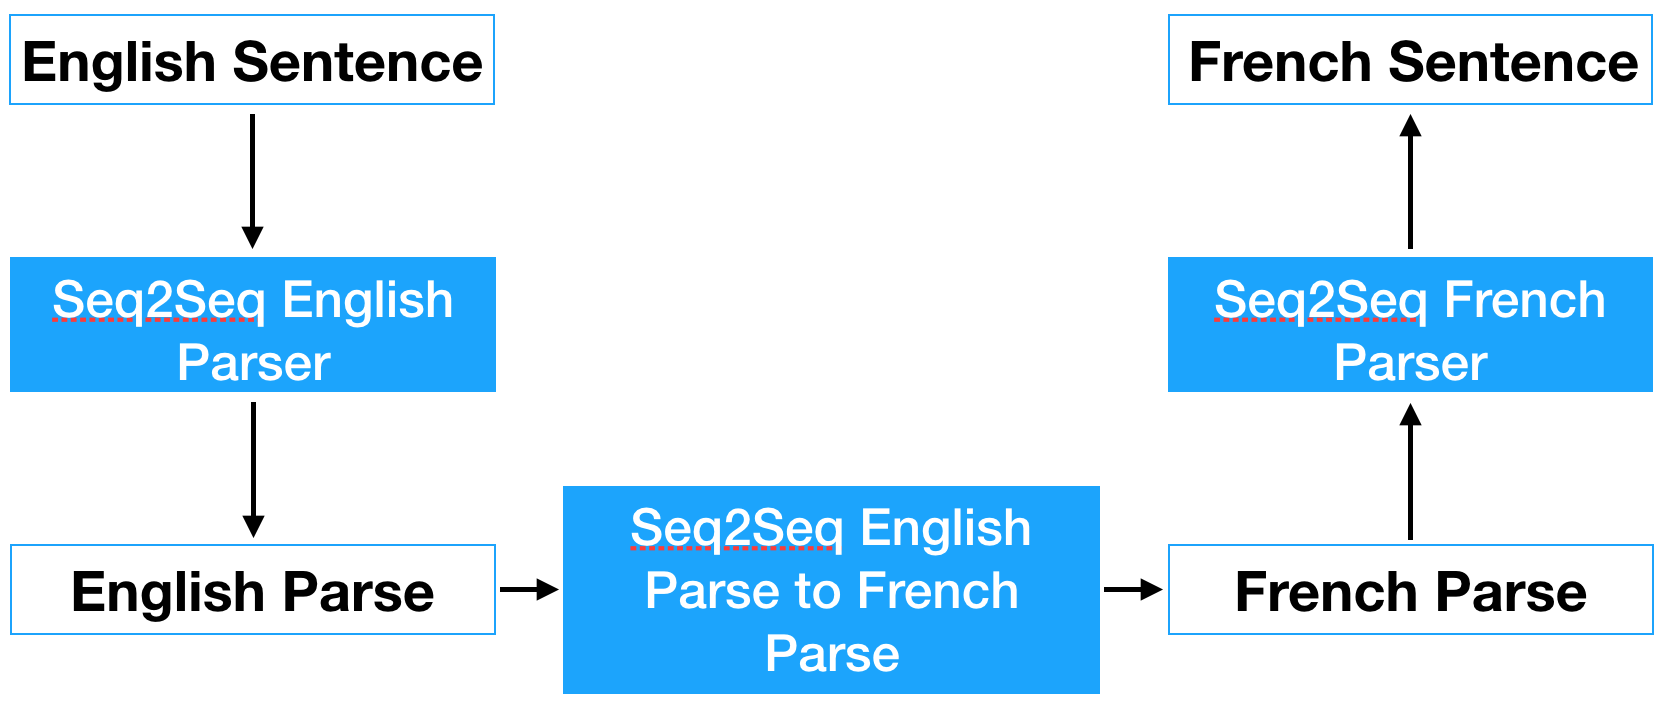
\includegraphics[trim=0 0 0 0, clip, width=3.25in]{architecture.png} \\
        Proposed Architecture\\
    \end{tabular}
    \label{fig:architecture}
\end{figure}

\section{Extensions}
Time-permitting, variations of the proposed model could be attempted. One idea is removing the section of the network that translates the French parse to the French sentence. This would mean that the network would need to translate directly from the English parse to the French sentence. This extension could be compared to the originally proposed architecture to see if one works better than the other.

Additionally, rather than training each of the network components separately then fine-tuning the whole network, I could try training the entire network from scratch. It would be interesting to see what kind of intermediate representations emerge at the section of the network where normally the parses would be.

\section{Dataset}
One challenge in this project will be in finding a dataset that not only has language to language translations, but also has accurate parses for each of the training sentences. I am unaware of any datasets that contain both these qualities. The Geoquery dataset contains English parses of sentences, and the Europarl parallel corpus \cite{Europarl} contains English to many other different language translations. If I cannot find a dataset that contains both these properties, I could pre-train a parser on English, pre-train a parser on another language (such as French), then train the entire network together using the English-French language pairs.

%------------------------------------------------------------------------------


{\small
\bibliographystyle{ieee}
\bibliography{proposal}
}

\end{document}
